%allgemeine Formatangaben
\documentclass[
 a4paper, 										% Papierformat
 12pt,												% Schriftgröße
 ngerman, 										% für Umlaute, Silbentrennung etc.
 titlepage,										% es wird eine Titelseite verwendet
 oneside, 										% einseitiges Dokument
 captions=nooneline,					% einzeilige Gleitobjekttitel ohne Sonderbehandlung wie mehrzeilige Gleitobjekttitel behandeln
 numbers=noenddot,						% Überschriften-??Nummerierung ohne Punkt am Ende
 parskip=half,									% zwischen Absätzen wird eine halbe Zeile eingefügt
 ]{scrartcl}


% Anpassung an Landessprache
\usepackage[ngerman]{babel}	

\usepackage[T1]{fontenc}	
\usepackage[utf8]{inputenc}	
\usepackage{textcomp} 																% Euro-Zeichen und andere
\usepackage[babel,german=quotes]{csquotes}						% Anführungszeichen
\RequirePackage[ngerman=ngerman-x-latest]{hyphsubst} 	% erweiterte Silbentrennung

\usepackage{tocloft} %Wird benötigt damit das veränderte Counterverhalten nicht mit Text überlappt!
\usepackage{etoolbox} %Url Umbruch im Bibtex!

% Befehle aus AMSTeX für mathematische Symbole z.B. \boldsymbol \mathbb
\usepackage{amsmath,amsfonts}

% Zeilenabstände und Seitenränder 
\usepackage{setspace}
\usepackage{geometry}

% Einbinden von JPG-Grafiken
\usepackage{graphicx}

% zum Umfließen von Bildern
% Verwendung unter http://de.wikibooks.org/wiki/LaTeX-Kompendium:_Baukastensystem#textumflossene_Bilder
\usepackage{floatflt}

% Verwendung von vordefinierten Farbnamen zur Colorierung
% Palette und Verwendung unter http://kitt.cl.uzh.ch/kitt/CLinZ.CH/src/Kurse/archiv/LaTeX-Kurs-Farben.pdf
\usepackage[usenames,dvipsnames]{color} 

% Tabellen
\usepackage{array}
\usepackage{longtable}

% einfache Grafiken im Code
% Einführung unter http://www.math.uni-rostock.de/~dittmer/bsp/pstricks-bsp.pdf
%\usepackage{pstricks}


% Quellcodeansichten
%\usepackage{verbatim}
%\usepackage{moreverb} 											% für erweiterte Optionen der verbatim Umgebung
% Befehle und Beispiele unter http://www.ctex.org/documents/packages/verbatim/moreverb.pdf
%\usepackage{listings} 											% für angepasste Quellcodeansichten siehe
% Kurzeinführung unter http://blog.robert-kummer.de/2006/04/latex-quellcode-listing.html



% verlinktes und Farblich angepasstes Inhaltsverzeichnis
\usepackage[pdftex,
colorlinks=true,
linkcolor=InterneLinkfarbe,
urlcolor=ExterneLinkfarbe]{hyperref}
\usepackage[all]{hypcap}

% URL verlinken, lange URLs umbrechen
\usepackage{url}

% sorgt dafür, dass Leerzeichen hinter parameterlosen Makros nicht als Makroendezeichen interpretiert werden
\usepackage{xspace}

% Beschriftungen für Abbildungen und Tabellen
%\usepackage{caption}

%\usepackage{chngcntr}
%Ändert counterverhalten von figure, table usw..

% Entwicklerwarnmeldungen entfernen
%\usepackage{scrhack}
% Glossar und Abbildungsverzeichnis
%\usepackage[
%nonumberlist, %keine Seitenzahlen anzeigen
%acronym,      %ein Abkürzungsverzeichnis erstellen
%toc          %Einträge im Inhaltsverzeichnis
%]      %im Inhaltsverzeichnis auf section-Ebene erscheinen
%{glossaries}
\usepackage{makeidx}
\makeindex

\usepackage{amsmath, amssymb}

\usepackage[printonlyused]{acronym}					% einbinden der verwendeten Latex-Pakete
\newcommand{\qq}[1]{\glqq{#1\grqq{}}} %Gänsefüßchen
\newcommand{\idx}[1]{#1\index{#1} } % Index drucken und schreiben

\onehalfspacing 							% 1,5facher Zeilenabstand

\definecolor{InterneLinkfarbe}{rgb}{0.1,0.1,0.3} 	% Farbliche Absetzung von externen Links
\definecolor{ExterneLinkfarbe}{rgb}{0.1,0.1,0.7}	% Farbliche Absetzung von internen Links

% Einstellungen für Fußnoten:
\captionsetup{font=footnotesize,labelfont=sc,singlelinecheck=true,margin={5mm,5mm}}

% Quellenangaben Stil
\bibliographystyle{alphadin}

%Ausschluss von Schusterjungen
\clubpenalty = 10000
%Ausschluss von Hurenkindern
\widowpenalty = 10000


% Beispiel für eine Listings-Codeumbebungen
% Bei mehreren Definitionen empfielt sich das auslagern in eine externe Datei
\lstloadlanguages{C++}
\lstset{
	frame=tb,
	framesep=5pt,
	basicstyle=\footnotesize\ttfamily,
	showstringspaces=false,
	keywordstyle=\ttfamily\bfseries %\color{CadetBlue},
	identifierstyle=\ttfamily,
	stringstyle=\ttfamily %\color{OliveGreen},
	%commentstyle=\color{GrayBlue},
%	rulecolor=\color{Gray},
	xleftmargin=5pt,
	xrightmargin=5pt,
	aboveskip=\bigskipamount,
	belowskip=\bigskipamount
} 

%Den Punkt am Ende jeder Beschreibung deaktivieren
\renewcommand*{\glspostdescription}{}

\setlength{\cftfignumwidth}{3em} %Befehl von tocloft
\setlength{\cfttabnumwidth}{3em}
%Counter verhalten verändern
\counterwithin{figure}{section}
\counterwithin{table}{section}

%Glossar-Befehle anschalten
\makeindex
\makeglossaries
\glsenablehyper

\apptocmd{\UrlBreaks}{\do\f\do\m}{}{}
			
\usepackage{tikz}			
\usetikzlibrary{shapes,arrows} %PAP
\begin{document}


\title{Entwicklung eines IR-Empfänger und -Sender mit dem ESP8266}
\subtitle{Dokumentation: Mikrocontroller-Anwendungs-Projekt}
\author{} %TODO Später hinzufügen
\date{\today}

\maketitle

\tableofcontents										% Inhaltsverzeichnis
\pagebreak
%\listoffigures											% Abbildungsverzeichnis
%\pagebreak
%\listoftables											% Tabellenverzeichnis
%\pagebreak

\section{Einleitung}
\subsection{Ausgangspunkt}
Der Ausgangspunkt des Projektes ist die Absicht eine Infrarotfernbedingung mit Hilfe eines Mikrocontrollers zu realisieren. Im Rahmen des aktuellen Hype um \acs{IoT} stellt diese Anforderung für uns eine interessante Möglichkeit da, bisher nicht \acs{IoT} fähige, über Infrarotfernbedienung gesteuerten Geräten diese Funktion \qq{nachzurüsten}. Hierdurch soll die Ansteuerung der Geräte wesentlich individueller belegbar sein, ohne dass, wie in anderen schon vorhanden Lösungen, (z.B. Logitech Harmony\footnote{ \url{http://www.logitech.com/de-de/harmony-remotes} ; Stand: \today}) eine neue Fernbedienung die alte ersetzt. Vielmehr soll ein schon vorhandenes Gerät/vorhandene Geräte diese Aufgabe mit übernehmen können.

Zur Umsetzung dieses Vorhabens bietet sich der Mikrocontroller ESP8266 an.
Er ist preiswert und besitzt ein integriertes WLAN-Modul.

\subsection{Ziele}
Ziel des Projektes ist es, eine Schaltung einschließlich dazugehöriger Mikrocontroller-Software zu entwickeln, die folgende Funktionen bietet:

\begin{itemize}
	\item Mikrocontroller muss die Dienste eines Webservers bereitstellen
	\item Kommunikation mit ESP8266 über drahtloses Netzwerk
	\item AccessPoint zur Konfiguration des ESP8266
	\item Einwahl in vorhandenes drahtloses Netzwerk und Speichern der Einwahldaten
	\item Steuerung des ESP8266 über Website
	\item Erfassen, Speichern und Ausgabe von Infrarot-Signalen (38kHz)
\end{itemize}

Alle diese Ziele sind mit Hilfe eines ESP8266 und weiterer Komponenten realisierbar.

\section{Grundlagen}
\subsection{Der ESP8266}
Der ESP8266 ist ein kostengünstiges, programmierbares \ac{SoC} mit einer \acs{WLAN}, \acs{UART}-und \acs{SPI}-Schnittstelle.
Ursprünglich wurde dieser \acs{SoC} von Espressif (daher ESP) entwickelt und verkauft, inzwischen bieten aber verschiedene andere Hersteller ebenfalls Varianten vom ESP8266 bzw. dem erweiterten ESP8266EX an.
Diese sind ab einem Stückpreis von ca. 2,00 € z.B. über AliExpress\footnote{\url{http://www.aliexpress.com} ; Stand: \today} verfügbar.

Nachfolgend ist die Spezifikation eines ESP8266 laut Espressif\footnote{\url{http://www.mikrocontroller.net/articles/ESP8266} ; Stand: \today} gelistet:

\begin{itemize}
    \item Wi-Fi Standards: 802.11 b/g/n, Wi-Fi Direct (\acs{P2P}), \acs{soft-AP}
    \item Integrierter TCP/IP Protokollstack
    \item Integrierter \acs{T/R} switch, \acs{balun}, \acs{LNA}, Leistungsverstärker
    \item Integrierte \acs{PLL}s, \acs{DCXO} und Spannungsversorgung
    \item +19.5dBm Ausgangsleistung im 802.11b Modus
    \item Power-Down Leckstrom <10$\mu$A
    \item Integrierte Verbrauchsarme 32-bit CPU (80 MHz)
    \item \acs{SDIO} 1.1/2.0, \acs{SPI}, \acs{UART}
    \item \acs{STBC}, 2×1 \acs{MIMO}
    \item \acs{A-MPDU} \& \acs{A-MSDU} \& 0.4ms Schutzintervalle
    \item Aufwachen und übermitteln von Paketen in < 2ms
    \item Standby Leistungsaufnahme < 1.0mW (\acs{DTIM3})
    \item\acs{VCC}: 3,3V (Nicht 5V tolerant)
    \item Flash Größe: 512kB - 4MB 
\end{itemize}

Verfügbare Flash-Größe, Arbeitsspeicher und CPU-Frequenz sind Modell und Hersteller abhängig. Häufig wird die versendete Form innerhalb des online Angebots nicht genauer beschrieben.

In der \autoref{fig:ESP8266} ist ein ESP8266 mit dem dazugehörigen Pinlayout dargestellt.

\begin{figure}
	\centering
	\begin{minipage}{0.45\textwidth}
			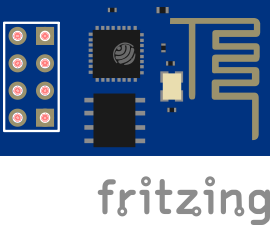
\includegraphics[scale=1.5]{Abbildungen/ESP8266A}
	\end{minipage}
	\hfill
	\begin{minipage}{0.45\textwidth} 
			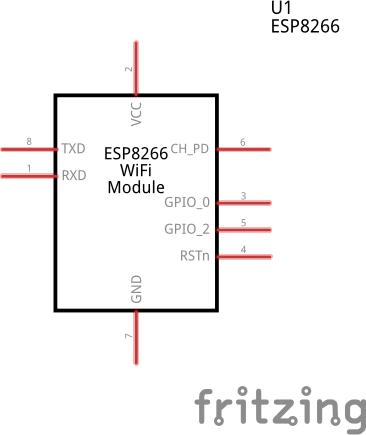
\includegraphics[scale=1.5]{Abbildungen/ESP8266}
	\end{minipage}
	\caption{ESP8266 Platine und Schaltung}
	\label{fig:ESP8266}
\end{figure}

\subsection{Programmierung}
Die Programmierung des Mikrocontrollers kann mit der Arduino IDE\footnote{\url{https://www.arduino.cc/} ; Stand: \today} erfolgen. Hierzu muss das Community Package esp8266 installiert sein, welches zusätzliche Header und Funktionen, sowie Compiler und Programmierdefinitionen beinhaltet.
In der IDE kann mit einer C/C++-Syntax programmiert werden, wobei der Compiler einige, aber nicht alle Befehlssätze des C++11 Standards unterstützt.

Weiterhin wird der ESP8266 über die \acs{TXD}- und \acs{RXD}-Leitungen mit Hilfe des \acs{UART}-Protokolls programmiert.
Damit der Controller in den Programmiermodus wechselt, muss beim Start der \acs{GPIO}\_0 auf Masse liegen (Controller startet im Programmiermodus).
Anschließend kann die durch Cross-Compiling erzeugte Binary von der Arduino IDE an den ESP8266 übertragen werden.
Für die Programmierung bieten sich beispielsweise sogenannte USB-to-\acs{UART}-Programmierkabel an (z.B. der PL2303).
Hierbei ist zu beachten, dass die Spannungsversorgung am Ausgang der meisten Programmierkabel 5V und nicht 3.3V beträgt. Der Mikrocontroller ist nicht 5V tolerant.

\subsection{Funktionsweise Fernbedienung}
%TODO Ausreichend?
%Damit eine WLAN-gesteuerte Infrarotfernbedingung realisiert werden kann, müssen zunächst die Grundlagen einer solchen Fernbedingung kurz erklärt werden.

Eine übliche Infrarot-Fernbedienung sendet ein Signal welches bei den meisten Herstellern von Fernsehern auf eine Trägerfrequenz von 36 - 38 kHz moduliert ist.
%Dieses Signal wird mit einer bestimmten Trägerfrequenz gesendet.
%Viele Fernbedingungen arbeiten beispielsweise mit einer Trägerfrequenz von 38kHz.
%Es existieren aber Fernbedingungen, welche andere Frequenzen nutzen.
In diesem Projekt wird eine Fernbedingung mit 38kHz realisiert. Bei genügend hoher Toleranz können hiermit aber auch Empfänger gesteuert werden welche ein 36 kHz Signal erwarten.
Es ist jedoch wichtig sich auf eine Frequenz festzulegen, da die Frequenz Einfluss auf Bauteile und Programmierung hat.

Über eine \ac{PWM} auf der Trägerfrequenz wird das codierte Signal übertragen.
Jede Taste auf einer Fernbedingung besitzt eine eigene Codierung.
Weiterhin existieren verschiedene Protokolle zur Codierung von Signalen.
Die Protokolle werden in diesem Projekt vernachlässigt, da die Codierung im Wesentlichen nur kopiert und gespeichert wird.

Damit das Infrarotsignal empfangen werden kann, wird ein entsprechender Empfänger benötigt.
Solche Empfänger sind als integrierte Schaltkreise verfügbar, welche alle benötigten Funktionen in einem Bauteil vereinen.
Ein Infrarotempfänger besteht aus einer Fotodiode, einem geregeltem Verstärker, welcher entsprechend der Frequenz arbeitet (zum Beispiel 38kHz) und einem Demodulator.
Der Demodulator sendet das digital codierte Signal an den Mikrocontroller.
Weiterhin besitzt der integrierte Schaltkreis einen Bandpassfilter um Störungen von anderen Frequenzen als der gewünschten Frequenz zu vermeiden.
Meist sind Fotodiode und Schaltkreis in einem Kunststoffgehäuse integriert.
Wir haben uns für den TSOP4836 entschieden, da dieser auf 38 kHz abgestimmt ist. Weitere Trägerfrequenzen sind in gleicher Bauform erhältlich.

Datenblatt: \url{http://mkpochtoi.narod.ru/TSOP4836_ds.pdf}\footnote{Stand: \today}

Auf die konkreten Details zu PWM wird in dieser Dokumentation nicht eingegangen.

\section{Realisierung}
Nachdem die Grundlagen für das Projekt betrachtet wurden, soll nun die konkrete Realisierung des Projektes verdeutlicht werden.
\subsection{Komponentenliste}
%TODO Liste
Für die Realisierung des Projektes werden folgenden Komponenten benötigt:
\begin{itemize}
	\item Der Mikrocontroller: ESP8266
	\item Ein Spannungsregler: LM1117-3V3
	\item Infrarotleuchtdiode: 1,5V / 80mA
	\item Vorwiderstand für Diode: 22 Ohm
	\item Infrarotempfänger: TSOP4836 für die Trägerfrequenz 38kHz
	\item USB-to-UART-Programmierer: PL2303
\end{itemize}


\subsection{Aufbau}
%TODO Vollständig?

Die \autoref{fig:Schalplan} zeigt den Schaltplan für die Realisierung einer Infrarotfernbedingung inklusive Empfänger.

\begin{figure}
	\centering
	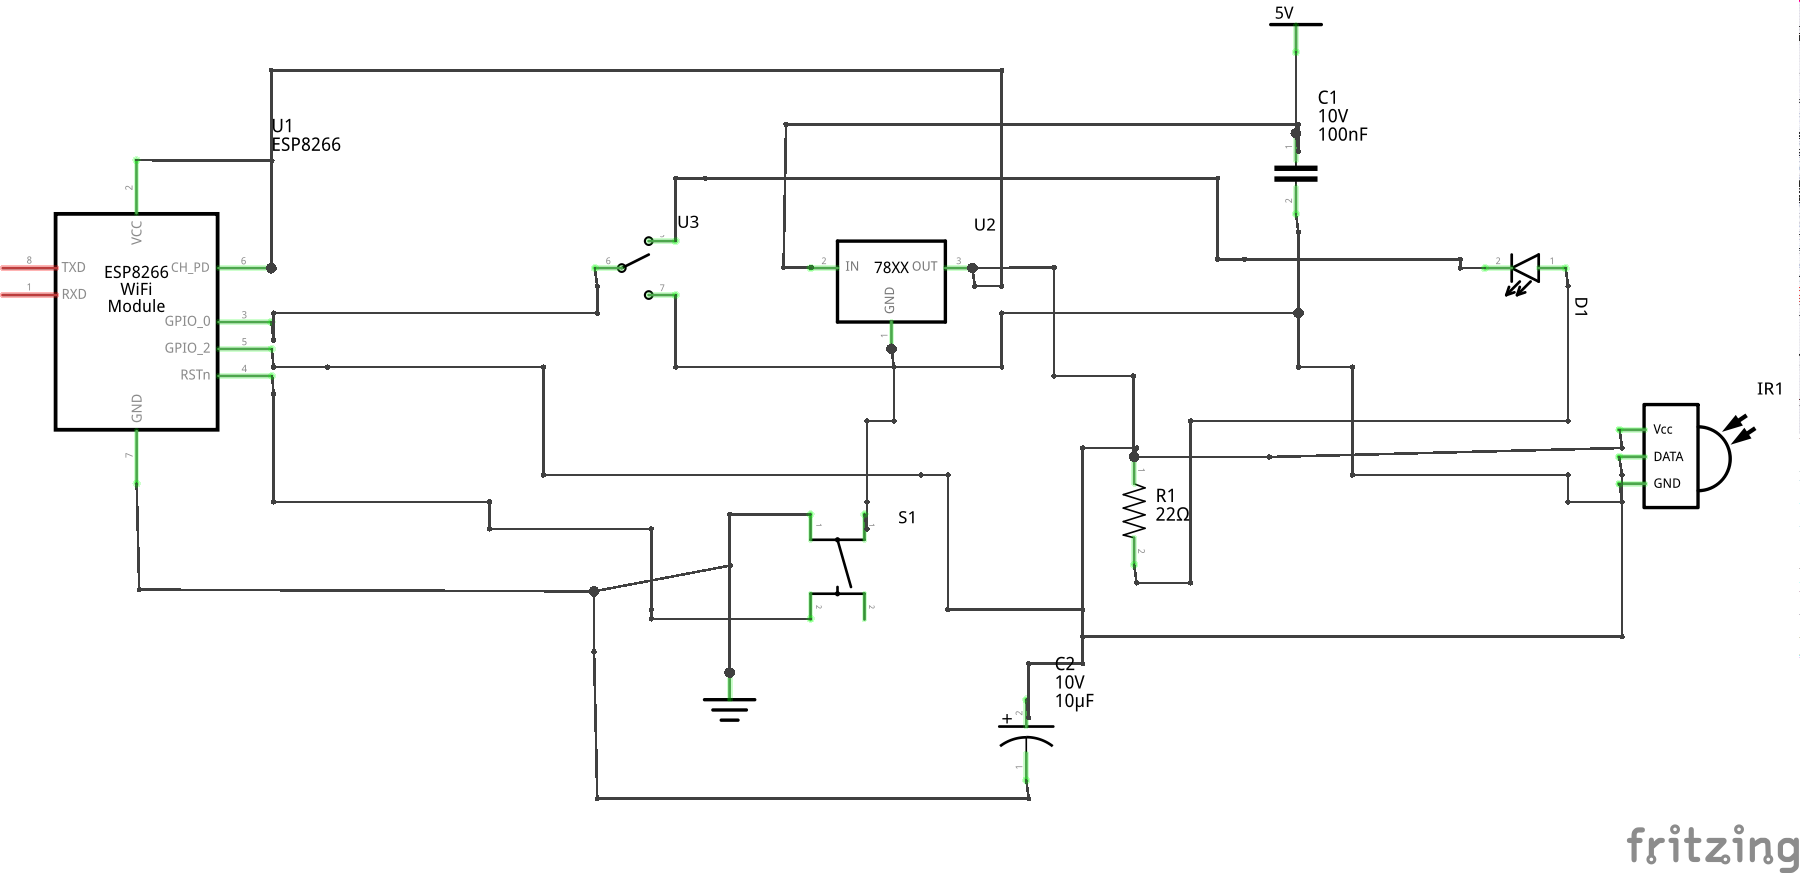
\includegraphics[scale=1.4]{Abbildungen/ESP8266_Schaltplan}
	\caption{Schaltplan}
	\label{fig:Schalplan}
\end{figure}

Für die Programmierung des Mikrocontrollers wird ein USB-to-UART-Programmierer (PL2303) verwendet.
Dieser liefert an VCC 5V. Wird er ohne PC betrieben kann er über ein einfaches 5V USB Netzteil auch als Zuleitung verwendet werden. Die TX und RX-Leitungen liegen dann auf 0V.
Der ESP8266 selbst benötigt 3,3V und ist nicht 5V tolerant, sodass ein Festspannungsregler verwendet wird um 3,3V für den Mikrocontroller zur Verfügung zu stellen.
Als Spannungsregler bietet sich zum Beispiel der LM1117-3V3\footnote{\url{http://www.ti.com/lit/ds/symlink/lm1117.pdf} ; Stand: \today} (verwendet) oder ein L7805 an.
Der Spannungsregler ist im Schaltplan als 78XX dargestellt.
Zur Spannungsstabilisierung wird dem Regler ein 100 nF Kondensator vor und ein Masse einen 10$\mu$F-Kondensator nachgeschaltet.

Nun wird für den ESP8266 die benötigte Spannung von 3,3V bereitgestellt.
Die Pins \acs{VCC} und \acs{CHPD} werden mit der Spannungsquelle 3,3V verbunden und \ac{GND} entsprechend auf Masse gelegt.
Der \acs{RST}-Pin wird mit einem Taster verbunden, welcher bei betätigen diesen Pin auf Masse zieht (interner Pull Up) und somit den Mikrocontroller zurücksetzt.

Das ESP8266-Modul besitzt 2 Digitale Ein beziehungsweise Ausgänge. \acs{GPIO}\_0 benutzen wir als Ausgang und \acs{GPIO}\_2 benutzen wir als Eingang.
Wie diese Pins arbeiten wird bei der Programmierung festgelegt.

An dem {GPIO}\_0 ist ein DIP-Schalter angeschlossen.
Dieser dient dazu zwischen dem Programmiermodus und dem normalen Modus zu Wechseln.
Der Pin ist Low-Aktiv, sodass für den normalen Betrieb und nach einem Reset immer 3,3V anliegen muss.
Für das Programmieren wird dieser Pin auf Masse gezogen in dem der Schalter entsprechend gesetzt wird und ein Reset ausgeführt wird.
Andernfalls ist der DIP-Schalter mit einer Infrarotdiode (1,5V, 80mA) inklusive Vorwiederstand(22 Ohm) verbunden.
Die Diode und der Widerstand sind mit der 3,3V Spannungsquelle verbunden.
Diese Diode dient später dazu die Infrarotsignale zu senden.

Der \acs{GPIO}\_0 2 wird mit dem Infrarotempfänger verbunden und dient zur Erfassung der Infrarot-Signale.
Der Infrarotempfänger wird entsprechend mit der 3,3V Spannungsquelle und der Masse verbunden.

Aufgrund dessen, dass Senden und Empfangen nicht gleichzeitig möglich sind, bedarf es keiner Abschirmung zwischen Sende und Empfangsdiode. Es wird über die Programmierung sichergestellt das der Sender während des erwarteten Aufnehmens von Signalen nicht Leuchtet (Ausgang liegt auf High).

Die \autoref{fig:Steckplatine} zeigt den Aufbau auf einer Steckplatine.

\begin{figure}
	\centering
	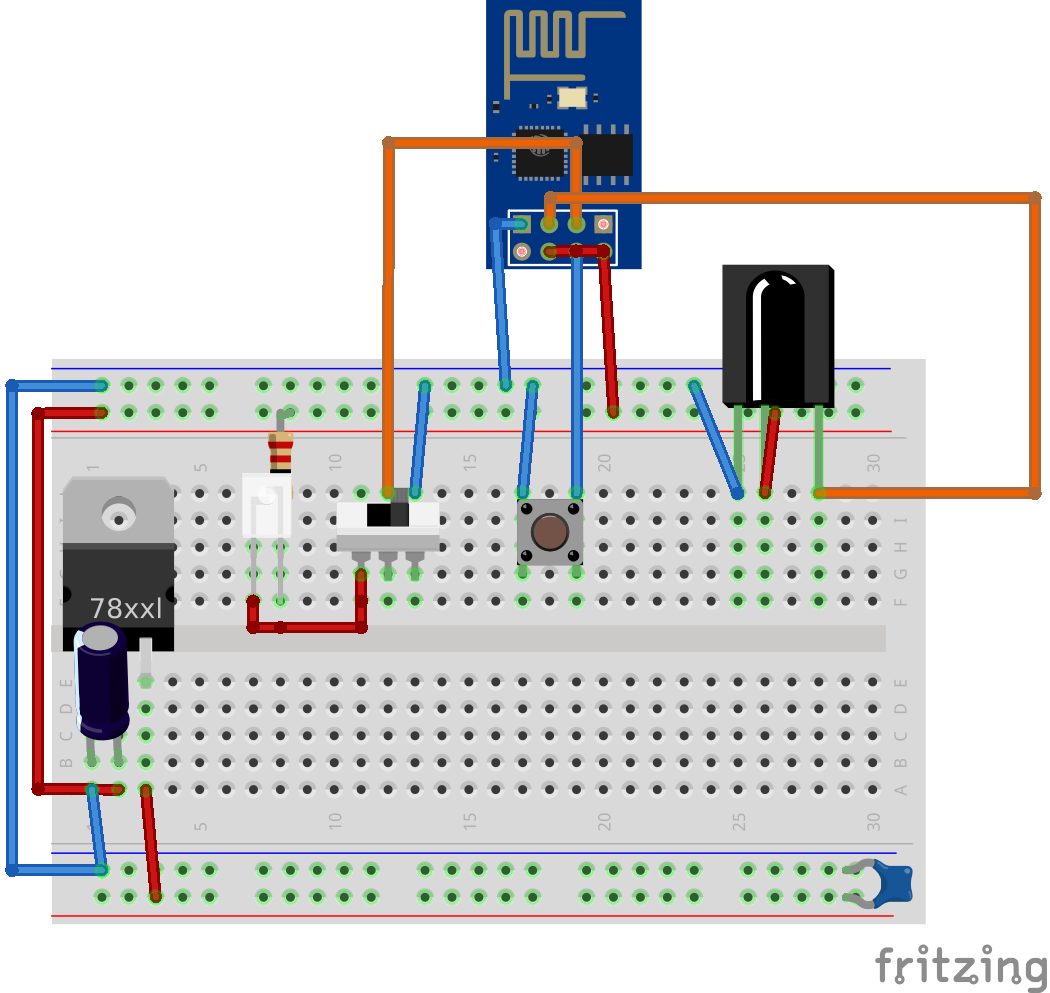
\includegraphics[scale=1]{Abbildungen/ESP8266_Steckplatine}
	\caption{Steckplatine}
	\label{fig:Steckplatine}
\end{figure}



\subsection{Implementierung}
%TODO vervollständigen
Ein Programm für den ESP8266 besteht aus 2 Teilen.
Diese 2 Teile sind jeweils definiert durch die Funktionen \texttt{setup()} (Initialisierung des Mikrocontrollers) und \texttt{loop()} (Schleife).

In der Funktion \texttt{setup} werden Befehle ausgeführt, welche beim Starten des Mikrocontrollers aufgerufen werden sollen.
Zum Beispiel ist es möglich im Setup eine Verbindung zum einem drahtlosen Netzwerk herzustellen und Serverfunktionalität bereitzustellen.
Nach Abschluss des Setups gelangt der Mikrocontroller in die \texttt{loop}-Funktion.
Diese Funktion wird beständig immer wieder aufgerufen und entsprechende entsprechende Befehle in der Funktion ausgeführt.
Zum Beispiel wird an dieser Stelle geprüft ob ein Client eine Anfrage an den Mikrocontroller gesendet hat.
Falls ja, werden die entsprechenden Funktionen ausgeführt.

\subsubsection{Programmablaufplan}
%TODO PAP für loop (übersichtlicher, wenn getrennt)
%beispiel: http://www.texample.net/tikz/examples/simple-flow-chart/

% Define block styles
\tikzstyle{decision} = [diamond, draw, 
    text width=4.5em, text badly centered, node distance=3cm, inner sep=0pt]
\tikzstyle{block} = [rectangle, draw, 
    text width=5em, text centered, rounded corners, minimum height=4em]
\tikzstyle{line} = [draw, -latex']
\tikzstyle{cloud} = [draw, ellipse, node distance=3cm,
    minimum height=2em]

\begin{center} 
\begin{tikzpicture}[node distance = 2cm, auto]
    % Place nodes
    \node [block] (init) {Start};
    \node [block, below of=init] (confPin) {Konfiguriere GPIOs};
    \node [cloud, left of=init] (setup) {Setup( )};
    \node [block, below of=confPin] (readIR) {Lese Infrarot-\footnotemark};
    \node [block, below of=readIR] (readWLAN) {Lese WLAN-\footnotemark[\value{footnote}]};
    \node [block, below of=readWLAN] (connectWLAN) {Verbinde mit WLAN};
    \node [decision, below of=connectWLAN] (decide) {Erfolgreich ?};
   	\node [block, left of=decide, node distance=4cm] (startAP) {Starte als AP};
    \node [block, below of=decide, node distance=3cm] (mDNS) {Starte \acs{mDNS}};
 	\node [block, below of=mDNS] (launch) {Starte Server};
    \node [block, below of=launch] (ende) {Ende};
    \node [cloud, right of=ende] (loop) {Loop( )};
    % Draw edges
    \path [line] (init) -- (confPin);
    \path [line] (confPin) -- (readIR);
    \path [line] (readIR) -- (readWLAN);
    \path [line] (readWLAN) -- (connectWLAN);
    \path [line] (connectWLAN) -- (decide);
	\path [line] (decide) -- node [near start] {Nein} (startAP);
    \path [line] (startAP) |- (launch);
    \path [line] (decide) -- node {Ja}(mDNS);
    \path [line] (mDNS) -- (launch);
    \path [line] (launch) -- (ende);
    \path [line,dashed] (setup) -- (init);
    \path [line,dashed] (ende) -- (loop);
\end{tikzpicture}
\footnotetext{Daten aus Speicher des ESP8266}
\end{center}

%TODO Noch zu vervollständigen

\subsubsection{Infrarotsignale Empfangen}
%TODO erklären ?? Wie funktioniert das? (Eike)
\subsubsection{Infrarotsignale Senden}
Damit Infrarotsignale mit einer Trägerfrequenz von 38kHz gesendet werden, bedarf es einem Trick in der Programmierung um dies zu realisieren.
Dies geschieht in dem der digitale Ausgang \acs{GPIO}\_2 zwischen einer logischen 1 und 0 alterniert.
Die Länge des Pulses beschreibt den gesendeten Befehl an den Infrarotempfänger.

Dies kann mit Hilfe eines $\mu$s-delay Befehl realisiert werden.
Jeder Puls ist 1/38000 Sekunden (26,3 $\mu$s) lang. Die restlichen 0.3 $\mu$s werden ca. von den Ansteuerungfunktionen für das Wechseln zwischen HIGH und LOW des Ausgangs so wie der Schleife verwendet.
Gerundet auf 26 $\mu$s ist die Modulationsfrequenz realisierbar mit:
%TODO Pseudocode wenn fertig

\subsection{Verwendung}
%TODO Screenshots browser (wäre cool, wenn du das machst Eike.., da bei mir der Mikrocontroller nachwievor rumzickt..) , verwendung beschreiben
%TODO Herr Bastian mag es, wenn ALLES gelernte in das Fazit / Zusammenfassung einfließt-> Fazit darf ruhig mehrere Seiten lang sein!!
%TODO Bitte ergänze das hier bitte mit @ Eike
%TODO Vervollständigen
\section{Fazit}

Im Verlaufe des Projektes ist ein über ein drahtloses Netzwerk steuerbare Mikrocontroller-Anwendung entstanden, welcher in einem heimischen Netzwerk verwendet werden kann.

Erworbene Fertigkeiten:
\begin{itemize}
	\item Programmierung in einer Arduino IDE inklusive entsprechender Konfiguration der IDE
	\item Programmierung in C/C++
	\item Umgang mit dem ESP8266
	\item Erworbenes Verständnis für die Funktionsweise von Infrarotsendern und Empfängern
\end{itemize} 

Es ist in der gewählten Realisierung nicht möglich die Stromsparmaßnahmen des Mikrocontrollers zu verwenden, da hierbei die WLAN Eigenschaften unterbrochen werden. Der Mikrocontroller kann dann nicht auf einkommende Anfragen reagieren und diese laufen in einen Timeout.

Der Quellcode für das Projekt ist auf GitHub verfügbar unter:\\ \url{https://github.com/Ava-chan/IOT_IR_Remote}\footnote{Stand: \today}

\pagebreak

\begin{appendix}
\pagestyle{empty}	
\section{Abkürzungsverzeichnis}

\begin{acronym}
\acro{A-MPDU}{\textbf{A}ggregated \textbf{M}ac \textbf{P}rotocol \textbf{D}ata \textbf{U}nit}{ - Eine Funktion im Wlan-Standard 802.11e und 802.11n um bei einer einzelne Übertragung mehrere Pakete zu senden}
\acro{A-MSDU}{\textbf{A}ggregated \textbf{M}ac \textbf{S}ervice \textbf{D}ata}{ - Eine Funktion im Wlan-Standard 802.11e und 802.11n um bei einer einzelne Übertragung mehrere Pakete zu senden}
\acro{balun}{\textbf{bal}anced-\textbf{un}balanced}{ - Wandler zwischen symmetrischen und unsymmetrischen Leistungssystemen}
\acro{CHPD}{\textbf{C}hip \textbf{P}ower \textbf{D}own}{ -Der Chip kann mit Hilfe dieses Pins vollständig heruntergefahren werden}
\acro{DCXO}{\textbf{D}igitally \textbf{C}ontrolled \textbf{O}scillator}{ - digital gesteuerter Quarzoszillator}
\acro{DTIM3}{\textbf{D}elivery \textbf{T}raffic \textbf{I}ndication \textbf{M}essage}{- regelmäßiger Broadcast des Access Point um Wireless-Stationen aufzuwecken}
\acro{GND}{Ground}
\acro{GPIO}{\textbf{G}eneral \textbf{P}urpose \textbf{I}nput \textbf{O}utput}{ - Durch logische Programmierung kann PIN Verhalten als Eingang oder Ausgang definiert werden}
\acro{IoT}{\textbf{I}nternet \textbf{o}f \textbf{T}hings}{ - \qq{intelligente Gegenstände} unterstützen Menschen unmerklich}
\acro{LNA}{\textbf{L}ow \textbf{N}oise \textbf{A}mplifier}{ - Rausch armer Verstärker}
\acro{mDNS}{\textbf{m}ulticast \textbf{DNS}}{- Ist ein Konfigurationsloses Verfahren um Netzwerkadressen als Namen zu IP-Adressen aufzulösen, dieses Verfahren muss vom Client-System unterstützt werden}
\acro{MIMO}{\textbf{M}ultiple \textbf{I}nput \textbf{M}ultiple \textbf{O}utput}{ - Nutzung mehrerer Sende- und Empfangsantennen}
\acro{P2P}{\textbf{P}eer to \textbf{P}eer}{ - Direkte Endgerät zu Endgerät Kommunikation}
\acro{PLL}{\textbf{P}hase-\textbf{L}ocked \textbf{L}oop}{ - Damit ein konstantes abgeleitetes Signal zwischen einem äußeren Referenzsignal und Oszillator entsteht, wird solch eine Phasenregelschleife verwendet} 
\acro{PWM}{\textbf{P}uls-\textbf{W}eiten-\textbf{M}odulation}
\acro{RST}{Reset}{ -Setzt den Controller zurück, sodass dieser einen Neustart durchführt}
\acro{RXD}{\textbf{R}eceive \textbf{D}ata}{ - Eingehende Leitung für Daten}
\acro{soft-AP}{\textbf{soft}ware enabled \textbf{A}ccess \textbf{P}oint}{ - ein über Software erstellter Access Point, welcher auf einem Gerät erzeugt wird welches nicht speziell als Router gedacht ist}
\acro{SDIO}{\textbf{S}ecure \textbf{D}igital \textbf{I}nput \textbf{O}utput}{ - SD-Interface um Peripheriegeräte (z.B. Webcam, GPS, Ethernet, ...) anzusprechen}
\acro{SPI}{\textbf{S}erial \textbf{P}eripheral \textbf{I}nterface}{ - Synchroner serieller Datenbus}
\acro{SoC}{\textbf{S}ystem-\textbf{o}n-a-\textbf{C}hip}{ - Integration aller Systeme in einem Chip / einem Bauteil}
\acro{STBC}{\textbf{S}pace \textbf{T}ime \textbf{B}lock \textbf{C}oding}{ - Übertragungsverfahren in Funknetzwerken um mehrfach Daten über mehrere Antennen verteilt zu versenden}
\acro{T/R}{\textbf{T}ransmit / \textbf{R}eceive}{ - Versenden und Empfangen von Signalen}
\acro{TXD}{\textbf{T}ransmit \textbf{D}ata}{ - Ausgehende Leitung für Daten}
\acro{UART}{\textbf{U}niversal \textbf{A}synchronous \textbf{R}eceiver \textbf{T}ransmitter} { - digitale serielle Schnittstelle mit einem speziellen Protokoll}
\acro{VCC}{\textbf{V}oltage at the \textbf{C}ommon \textbf{C}ollector} { - Versorgungsspannung}
\acro{WLAN}{\textbf{W}ireless \textbf{L}ocal \textbf{A}rea \textbf{N}etwork}{ - engl. auch WiFi - kabellose Netzwerkverbindung}
\end{acronym}
\end{appendix}

\end{document}